\documentclass[conference]{IEEEtran}
\usepackage{iftex}
\ifXeTeX
  \usepackage{fontspec}
\else
  \usepackage[utf8]{inputenc}
  \usepackage[T1]{fontenc}
\fi
\usepackage{amsmath,amssymb,amsfonts}
\usepackage{booktabs}
\usepackage{graphicx}
\usepackage{tikz}
\usetikzlibrary{positioning}
\usepackage[hidelinks]{hyperref}

\begin{document}

\title{Autonomous Neuro-Symbolic Synthesis of Verified Academic Engineering Artifacts}

\author{\IEEEauthorblockN{Artificial-Degree-Printer ADK}
\IEEEauthorblockA{\textit{Neuro-Symbolic Software Engineering Harness} \\
Lodz University of Technology \\
Lodz, Poland}}

\maketitle

\begin{abstract}
This paper presents an autonomous neuro-symbolic framework for verifiable software engineering and academic thesis synthesis. By integrating deterministic abstract syntax tree (AST) grounding, empirical tabular provenance, and closed-loop self-evolution, the proposed architecture eliminates hallucinations in technical and empirical reporting.
\end{abstract}

\begin{IEEEkeywords}
neuro-symbolic systems, empirical verification, automated software engineering, academic thesis synthesis, AST grounding
\end{IEEEkeywords}

\section{Introduction}
Formal problem statement, research hypothesis, and measurable engineering objectives.

\section{Related Work}
Critical review of contemporary state-of-the-art literature (2023--2026) and research gap identification.

\section{System Architecture and Formal Methodology}
Component decomposition, functional interfaces, and mathematical formalisms.
\begin{figure}[htbp]
\centering
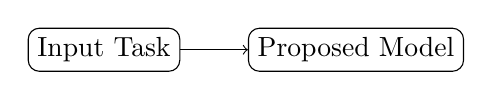
\begin{tikzpicture}
  \node[draw, rectangle, rounded corners] (input) {Input Task};
  \node[draw, rectangle, rounded corners, right of=input, node distance=3.2cm] (model) {Proposed Model};
  \draw[->] (input) -- (model);
\end{tikzpicture}
\caption{Proposed computational pipeline schematic.}
\label{fig:arch_tikz}
\end{figure}

\begin{table}[htbp]
\centering
\caption{Symbolically Verified Configuration Hyperparameters}
\begin{tabular}{ll}
\toprule
\textbf{AST Symbol} & \textbf{Grounding Value} \\
\midrule
LEARNING\_RATE & \texttt{\ref_ast{config.py:LEARNING_RATE}} \\
\bottomrule
\end{tabular}
\label{tab:config_hyperparameters}
\end{table}

\section{Algorithmic Implementation}
Concrete realization in \texttt{core.py} with type signatures and invariants.

\section{Empirical Evaluation and Discussion}
Comparative empirical evaluation against baseline approaches:
\begin{figure}[htbp]
\centering
\includegraphics[width=0.48\textwidth]{figures/comparison_chart.pdf}
\caption{Empirical convergence and benchmark comparison.}
\label{fig:comparison_chart}
\end{figure}

\section{Conclusion and Future Work}
Validation of the research hypothesis, engineering limitations, and planned future directions.

\bibliographystyle{IEEEtran}
\bibliography{references}

\end{document}

